\documentclass{beamer}
%pdflatex -shell-escape my_document.tex

\usetheme{default}
\usecolortheme{rose}
\usefonttheme{serif}
%\usefonttheme{structureitalicsserif}

\definecolor{verdeuni}{rgb}{0.7,0.73437,0.55856}
\setbeamertemplate{headline}[verdeuni]
%\setbeamercovered{highly dinamic}
%\usepackage{eso-pic}

\usepackage{minted}

\usepackage{stmaryrd}
\usepackage{local-macros2}
\newcommand{\distance}[2]{|#1 - #2|}
\newcommand{\outputdistance}[2]{||#1 - #2||}
%\newcommand{\x}{\vect{x}} 		% Arbitrary input
%\newcommand{\xt}{\hat{\x}} 		% Training input
\newcommand{\xs}{\x} 			% Sampled input
\newcommand{\xp}{\tilde{\x}} 	% Perturbed input

%\newcommand{\y}{\vect{y}} 		% Arbitrary output
\newcommand{\yt}{\hat{\y}} 		% Training output
\newcommand{\ys}{\y} 			% Sampled output



\newcommand{\SR}[2]{SR(#1, #2)} % Standard robustness
\newcommand{\LR}[2]{LR(#1, #2)} % Lipschitz robustness
\newcommand{\CR}[1]{CR(#1)} % Classification robustness
\newcommand{\SCR}[2]{SCR(#1,#2)} % Approximate class. robustness

\usepackage{amsfonts,amsmath,amssymb,amsthm}
\usepackage[all]{xy}
\usepackage{array,url}
\usepackage{textcomp,textgreek}
\usepackage{pgfplots}
\usepackage{float}
\pgfplotsset{width=5cm,compat=1.9}
\usepackage{mdframed,wrapfig,subcaption}
%\usepackage[font=footnotesize,labelfont=it
%\usepackage[latin1]{inputenc}
\usepackage{babel}
\usepackage{color}
%\usepackage{url}
\usepackage{hyperref}
\usepackage{fancyvrb}
%\usepackage{tikz}
\usepackage{alltt}
%\usepackage{etex, xy}
%\usepackage{cibeamer}
\usepackage{tikz}
\usetikzlibrary{arrows,shapes}
%\xyoption{all}
%\usepackage{listings}
%\input macro
\usepackage{cancel, comment}
\usepackage{verbatim}
\usepackage{slashbox}
\usepackage{ulem}

\newcommand{\tikzmark}[1]{\tikz[remember picture] \node[coordinate] (#1) {#1};}
\newcommand{\semitransp}[2][35]{\color{fg!#1}#2}

\usepackage[absolute,overlay]{textpos}
\beamertemplatenavigationsymbolsempty
\usepackage{ijcnn-diagram}

\usepackage[all]{foreign}

\newcommand{\fstar}{F$^\ast$\xspace}
\newcommand{\starchild}{StarChild\xspace}
\newcommand{\lazuli}{Lazuli\xspace}
\newcommand{\sapphire}{Sapphire\xspace}
\newcommand{\cL}{{\cal L}}
%\newcommand{\Real}{{\mathbb R}}
\usepackage{makecell}
\DeclareMathOperator{\linear}{linear}
\DeclareMathOperator{\relu}{relu}
\DeclareMathOperator{\sigmoid}{sigmoid}
\DeclareMathOperator{\softmax}{softmax}
\DeclareMathOperator{\neuron}{neuron}
\DeclareMathOperator{\truthy}{truthy}
\DeclareMathOperator{\falsey}{falsey}
\DeclareMathOperator{\neurontest}{test}
\usepackage{ellipsis}
\renewcommand{\ellipsisgap}{-0.25em}

\usepackage{soul}
\makeatletter
\let\HL\hl
\renewcommand\hl{%
  \let\set@color\beamerorig@set@color
  \let\reset@color\beamerorig@reset@color
  \HL}
\makeatother

%\usetikzlibrary{decorations.pathreplacing,shapes.arrows}
\newcommand\BackgroundPicture[1]{%
  \setbeamertemplate{background}{%
   \parbox[c][\paperheight]{\paperwidth}{%
      \vfill \hfill
\includegraphics[width=1\paperwidth,height=1\paperheight]{#1}
        \hfill \vfill
     }}}
\usepackage{xcolor,colortbl}
%\usepackage{listings}
\definecolor{Gray}{gray}{0.85}

%\setbeamertemplate{footline}[frame number]

%\newcommand{\rrdc}{\mbox{\,\(\Rightarrow\hspace{-9pt}\Rightarrow\)\,}} % Right reduction
%\newcommand{\lrdc}{\mbox{\,\(\Leftarrow\hspace{-9pt}\Leftarrow\)\,}}% Left reduction
%\newcommand{\lrrdc}{\mbox{\,\(\Leftarrow\hspace{-9pt}\Leftarrow\hspace{-5pt}\Rightarrow\hspace{-9pt}\Rightarrow\)\,}} % Equivalence
%\DeclareMathOperator{\id}{Id}
%\newcommand{\Zset}{\mathbb{Z}}
%\newcommand{\Bset}{\mathbb{Z}_2}

\setbeamertemplate{navigation symbols}{}

\mode<presentation>
\title[Vehicle Tutorial Chapter 1]{Vehicle Tutorial Chapter 1: Getting Started}
%\subtitle{in Neuro-Symbolic Landscape}
\author[Vehicle]{Ekaterina Komendantskaya and Matthew Daggitt (today's presentors), on behalf of the Vehicle team}
\institute[]{}

\date[]{}

%\logo{
\includegraphics[width=6cm]{LaivLogolong.png}}

\AtBeginSection[]
{
  \begin{frame}
    \frametitle{Table of Contents}
    \tableofcontents[currentsection]
  \end{frame}
}

\begin{document}
\BackgroundPicture{logo1.png}

\begin{frame}
\titlepage
\end{frame}

\begin{frame}
\frametitle{In this chapter...}

We will:

\begin{itemize}[<+->]
\item  ... introduce Main building blocks of Vehicle as a Programming Language
\item ... get to practice working with Vehicle
\item ... use the famous ACAS Xu benchmark to show Vehicle's work flow --
from specification to verification
\item ... identify PL problems (cf Introduction) that are resolved by Vehicle

\end{itemize}

\end{frame}


\begin{frame}
\frametitle{Recap: four PL problems}

\pause
\begin{itemize}
\item[$I^O$] Interoperability -- properties are not portable between training/counter-example search/ verification.

\item[$I^{P}$] Interpretability -- code is not easy to understand.

\item[$I^{\int}$] Integration -- properties of networks cannot be linked to larger control system properties.

\item[$E^G$] Embedding gap -- little support for translation between problem space (as in original spec) and input space (at neural network level).
\end{itemize}
\end{frame}


    \begin{frame}
\frametitle{Recap: ACAS Xu}
A collision avoidance system for unmanned autonomous aircraft.
\tikz [remember picture,overlay]{
\node at ([xshift=3cm,yshift=3cm]current page.south) {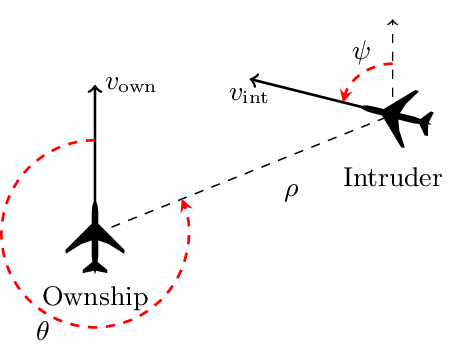
\includegraphics[width=0.5\linewidth]{Images/acas_xu.png}};}

{\small
Inputs:
\vspace{-0.7em}
\begin{itemize}
\setlength\itemsep{-0.1em}
\item Distance to intruder, $\rho$
\item Angle to intruder, $\theta$
\item Intruder heading, $\varphi$
\item Speed, $v_{own}$
\item Intruder speed, $v_{int}$
\end{itemize}


Outputs:
\vspace{-0.7em}
\begin{itemize}
\setlength\itemsep{-0.1em}
\item Clear of conflict
\item Strong left
\item Weak left
\item Weak right
\item Strong right
\end{itemize}}

\end{frame}


\begin{frame}
\frametitle{ACAS Xu}

%\pause
\begin{definition}[ACAS Xu: Property 3]
{\it If the intruder is directly ahead and is moving towards the
 ownship, the score for COC will not be minimal.}
\end{definition}

%\pause
\begin{block}{}
\begin{equation*}
\begin{array}{l}
1500 \leq \rho \leq 1800 \wedge -0.06 \leq \theta \leq 0.06 \\
 \wedge \psi \geq 3.10 \wedge v_{own} \geq 980 \wedge
v_{int} \geq 960 \\
\Rightarrow \text{the score for COC} \neq 0
%(\rho \geq 55947.691) \wedge
%(v_{own} \geq 1145) \wedge (v_{int} \leq 60)  \\
%\Rightarrow \text{the score for COC is at most 1500}
\end{array}
\end{equation*}
\end{block}

\end{frame}


\section{Vehicle' Syntax}

\begin{frame}[fragile]
\frametitle{Types}
Let us build the ACAS Xu specification.

We start with types of input and output vectors, as well as types of ACAS Xu networks

\begin{minted}[fontsize=\small]{vehicle}

type InputVector = Vector Rat 5
type OutputVector = Vector Rat 5

@network
acasXu : InputVector -> OutputVector
\end{minted}

\begin{block}{}

The Vector type represents a mathematical vector, or in programming terms can be thought of as a fixed-length array.
\end{block}
\end{frame}

\begin{frame}[fragile]
\frametitle{Values}

Types for values are automatically inferred by \textbf{Vehicle}. For example, we can declare the number $\pi$ and its type will be inferred as rational:

\begin{minted}[fontsize=\small]{vehicle}

pi = 3.141592
\end{minted}
\end{frame}

\begin{frame}[fragile]
\frametitle{Working with vectors}
\begin{itemize}
\item some input or output pre-processing maybe expected when defining a neural network.

\begin{example}
It is assumed that the ACAS Xu inputs and outputs are normalised, i.e. the network does not work directly with units like $m/s$. However, the specifications  we want to write should ideally concern the original units.
\end{example}

\pause


\item This is an instance of \emph{``problem space / input space mismatch"}

\item ... that is very common in neural net verification

\item
Being able to reason about problem space (alongside the input space) is a feature that distinguishes \textbf{Vehicle} from
majority of the mainstream neural network verifiers
\end{itemize}
\end{frame}

\begin{frame}[fragile]
\frametitle{Vector normalisation}
For clarity, we define a new type synonym for unnormalised input vectors which are in the problem space.
\begin{minted}[fontsize=\footnotesize]{vehicle}

type UnnormalisedInputVector = Vector Rat 5

\end{minted}

Next we define the range of the inputs that the network is designed
to work over.

\begin{minted}[fontsize=\footnotesize]{vehicle}

minimumInputValues : UnnormalisedInputVector
minimumInputValues = [0,0,0,0,0]

maximumInputValues : UnnormalisedInputVector
maximumInputValues = [60261.0, 2*pi, 2*pi, 1100.0, 1200.0]

meanScalingValues : UnnormalisedInputVector
meanScalingValues = [19791.091, 0.0, 0.0, 650.0, 600.0]
\end{minted}
\end{frame}

\begin{frame}[fragile]
\frametitle{Vector manipulation}
An alternative method to vector definition is to use the `foreach` constructor, which is used to provide a value for each `index i`.
\begin{minted}[fontsize=\footnotesize]{vehicle}

minimumInputValues : UnnormalisedInputVector
minimumInputValues = foreach i . 0

\end{minted}
Let us see how  `foreach` works with vector indexing.

We can now define the normalisation function that takes an input vector and
returns the unnormalised version.

\begin{minted}[fontsize=\footnotesize]{vehicle}

normalise : UnnormalisedInputVector -> InputVector
normalise x = foreach i .
  (x ! i - meanScalingValues ! i) / (maximumInputValues ! i)
\end{minted}

\pause
... our first acquaintance with functions!

\end{frame}

\begin{frame}[fragile]
\frametitle{Functions and types}
\begin{minted}[fontsize=\footnotesize]{vehicle}
<name> : <type>
<name> [<args>] = <expr>

\end{minted}
Functions make up the backbone of the \textbf{Vehicle} language.
\pause
\begin{minted}[fontsize=\footnotesize]{vehicle}

validInput : UnnormalisedInputVector -> Bool
validInput x = forall i .
  minimumInputValues ! i <= x ! i <= maximumInputValues ! i

\end{minted}

\pause

\begin{block}{Our first acquaintance with predicates and quantifiers!}
 One of the main advantages of \textbf{Vehicle} is that it can be used to state and prove specifications that describe the network’s behaviour over an infinite set of values.
\end{block}

\end{frame}


\begin{frame}[fragile]
\frametitle{Functions and types}

\begin{block}{Function Composition: Exercise}

What are the types of functions `acasXu`  and `normalise`:

\begin{minted}[fontsize=\footnotesize]{vehicle}
normAcasXu : UnnormalisedInputVector -> OutputVector
normAcasXu x = acasXu (normalise x)
\end{minted}
\end{block}

\end{frame}

\begin{frame}[fragile]
\frametitle{Pre-defined functions and predicates}
We have already used:
\begin{minted}[fontsize=\footnotesize]{vehicle}
*
/
!
<=
\end{minted}

\begin{block}{Exercise}
\footnotesize{What do they stand for?}
\end{block}
\end{frame}

\begin{frame}[fragile]
\frametitle{Lets verify ACAS Xu!}
\begin{minted}[fontsize=\footnotesize]{vehicle}
distanceToIntruder = 0   -- measured in metres
angleToIntruder    = 1   -- measured in radians
intruderHeading    = 2   -- measured in radians
speed              = 3   -- measured in metres/second
intruderSpeed      = 4   -- measured in meters/second

clearOfConflict = 0
weakLeft        = 1
weakRight       = 2
strongLeft      = 3
strongRight     = 4
\end{minted}
\footnotesize{
The fact that all vector types come annotated with their size means that it
 is impossible to mess up indexing into vectors, e.g. if you changed
 `distanceToIntruder = 0` to `distanceToIntruder = 5` the specification would
 fail to type-check.}



\end{frame}

\begin{frame}[fragile]
\frametitle{Property 3}


\footnotesize{\textbf{If the intruder is directly ahead and is moving towards the
 ownship, the score for COC will not be minimal.}}

\pause

\begin{minted}[fontsize=\footnotesize]{vehicle}
directlyAhead : UnnormalisedInputVector -> Bool
directlyAhead x =
  1500  <= x ! distanceToIntruder <= 1800 and
  -0.06 <= x ! angleToIntruder    <= 0.06
\end{minted}
\pause
\begin{block}{Exercise!}
\footnotesize{
\begin{enumerate}
\item
Can you identify whether the specification is written in terms of input space or problem space? How do you know?
\item Can you spot another pre-defined \textbf{Vehicle} function? What is it?
\end{enumerate}}
\end{block}

\end{frame}


\begin{frame}[fragile]
\frametitle{Property 3}

\footnotesize{\textbf{If the intruder is directly ahead and is moving towards the
 ownship, the score for COC will not be minimal.}}

\pause

\begin{minted}[fontsize=\footnotesize]{vehicle}
movingTowards : UnnormalisedInputVector -> Bool
movingTowards x =
  x ! intruderHeading >= 3.10  and
  x ! speed           >= 980   and
  x ! intruderSpeed   >= 960
\end{minted}
\pause
\begin{block}{Exercise!}
\footnotesize{
\begin{enumerate}
\item Can you spot one more pre-defined \textbf{Vehicle} function? What is it?
\end{enumerate}}
\end{block}

\end{frame}

\begin{frame}[fragile]
\frametitle{There is little left to do!}

\footnotesize{
\textbf{If the intruder is directly ahead and is moving towards the
 ownship, the score for COC will not be minimal.}}

\pause

\begin{minted}[fontsize=\footnotesize]{vehicle}
@property
property3 : Bool
property3 = forall x . validInput x and 
                       directlyAhead x and 
                       movingTowards x =>
  not (advises clearOfConflict x)
\end{minted}
\pause
\begin{block}{Exercise!}
\footnotesize{
\begin{enumerate}
\item Can you guess the purpose of the syntax
\begin{minted}{vehicle}
@property
\end{minted}
?
\item What kind of domain  `forall` ranges over? Is it finite or infinite?
\end{enumerate}}
\end{block}

\end{frame}

\begin{frame}[fragile]
\frametitle{How to run Vehicle}
\begin{block}{Checklist}
\begin{enumerate}
\item a verifier installed (Marabou);
\item the actual network is supplied in an ONNX format
\item \textbf{Vehicle} is installed.
\end{enumerate}
\end{block}

\pause
\begin{minted}[fontsize=\footnotesize]{vehicle}
vehicle verify \
  --specification acasXu.vcl \
  --verifier Marabou \
  --network acasXu:acasXu_1_7.onnx \
  --property property3

Verifying properties:
property3 [==========================================] 1/1 queries
  result:  counterexample found
  x: [1799.9886669999978, 1.9509286320000003e-2, 
                        3.09999732192, 980.0, 1017.6036]
\end{minted}
\end{frame}



\begin{frame}[fragile]
\frametitle{Exercise  1 (moderate): $\epsilon$-ball Robustness}
 \begin{minted}[fontsize=\tiny]{vehicle}
type Image = Tensor Rat [28, 28]
type Label = Index 10
validImage : Image -> Bool
validImage x = forall i j . 0 <= x ! i ! j <= 1

@network
classifier : Image -> Vector Rat 10

advises : Image -> Label -> Bool
advises x i = forall j . j != i => classifier x ! i > classifier x ! j

@parameter
epsilon : Rat

boundedByEpsilon : Image -> Bool
boundedByEpsilon x = forall i j . -epsilon <= x ! i ! j <= epsilon

robustAround : Image -> Label -> Bool
robustAround image label = forall pertubation .
  let perturbedImage = image - pertubation in
  boundedByEpsilon pertubation and validImage perturbedImage =>
    advises perturbedImage label

@dataset
trainingImages : Vector Image n

@dataset
trainingLabels : Vector Label n

@property
robust : Vector Bool n
robust = foreach i . robustAround (trainingImages ! i) (trainingLabels ! i)
\end{minted}
\end{frame}

\begin{frame}
\frametitle{Vehicle ...}

 \textbf{ the part that we have seen}

\begin{center}
\begin{tikzpicture}[thick,
    set/.style = {circle,
        minimum size = 3cm}]

% Set A
\node[rectangle,draw] (A) at (1.5,5) {\alert{\textbf{Property in Vehicle}}};

\node[rectangle,draw] (B) at (-3,2) {Training};
\node[text width=1cm, align=center] at (-3,0) {DL2 ACT etc.};

\node[rectangle,draw, dashed, text width=1.4cm] (C) at (0,2) {Counter-example search};
\node[text width=1cm, align=center] at (0,0) {PGD FGSM etc.};

\node[rectangle,draw] (D) at (3,2) {\alert{\textbf{Verification}}};
\node[text width=1.4cm, align=center] at (3,0) {\alert{\textbf{Marabou}} Eran etc.};

\node[rectangle,draw] (E) at (6,2) {Integration};
\node[text width=2cm, align=center] at (6,-0.3) {Agda Imandra KeymaeraX etc.};

\draw [->] (A) edge (B);
\draw [->, dashed] (A) edge (C);
\draw [->] (A) edge (D);
\draw [->] (A) edge (E);

\draw [->, dotted] (B) edge (C);
\draw [->, dotted] (C) edge (D);
\draw [->, dotted] (D) edge (E);

\onslide<1->{
\node[rectangle,draw,fill=normal text.bg] (D) at (1.5,4) {\alert{\textbf{Analysis \& informative error messages}}};
}

\end{tikzpicture}
\end{center}
\end{frame}

\begin{frame}
\frametitle{Concluding Exercise}

Which of the four PL problems we addressed?

\begin{itemize}
\item[$I^O$] Interoperability -- properties are not portable between training/counter-example search/ verification.

\item[$I^{P}$] Interpretability -- code is not easy to understand.

\item[$I^{\int}$] Integration -- properties of networks cannot be linked to larger control system properties.

\item[$E^G$] Embedding gap -- little support for translation between problem space (as in original spec) and input space (at neural network level).
\end{itemize}
\end{frame}

\begin{frame}[fragile]
\frametitle{Exercise  2 (hard): ACAS Xu: Property 1}

\small{
ACAS Xu Property 1 gives an idea how the {\it embedding gap} can arise not only when we reason about inputs, but also the outputs of networks!
%In the previous lecture, we introduced ACAS Xu property 1.

\begin{itemize}
\item Can you formalise Property 1 in Vehicle?
\item Can you spot the instance of the embedding gap, this time concerning the network's output?
\end{itemize}}

\pause

\begin{definition}[ACAS Xu: Property 1]
\small{\it If the intruder is distant and is significantly slower than the ownship, the score of a COC advisory will always be below a certain fixed threshold:}



\begin{equation*}
\begin{array}{l}
(\rho \geq 55947.691) \wedge
(v_{own} \geq 1145) \wedge (v_{int} \leq 60)  \\
\Rightarrow \text{the score for COC is at most} 1500
\end{array}
\end{equation*}
\end{definition}

\pause

\begin{block}{Note:}
The ACAS Xu neural network outputs are scaled as follows: given an element $x$ of the output vector, we scale it as: $\frac{x - 7.518884}{373.94992}$. 
\end{block}

\end{frame}

\end{document}
